\ifdefined\isinprint
\documentclass[twoside,10pt]{book}
\usepackage[twoside,paperwidth=155.93mm,paperheight=233.89mm,hmargin={15mm,15mm},vmargin={20mm,20mm},bindingoffset=5mm]{geometry}
\usepackage[hyphens]{url} 
\usepackage[colorlinks=false,
            pdfborder={0 0 0}
	        pdftex,
            plainpages=false,
            pdfauthor={Lukas Ladenberger (Editor)},
            pdftitle={BMotion Studio User's Handbook},
            pdfsubject={BMotion Studio},
            pdfkeywords={ProB, Event-B},
            pdfproducer={http://www.stups.hhu.de/ProB/index.php5/BMotion_Studio},
            pdfcreator={plastex-based tool chain}]{hyperref}
\else
\documentclass[12pt]{book}
\usepackage[left=2.5cm,top=3cm,right=2.5cm,bottom=3cm]{geometry}
\usepackage[hyphens]{url} 
\usepackage[colorlinks=true,
	        pdftex,
            plainpages=false,
            pdfauthor={Lukas Ladenberger (Editor)},
            pdftitle={BMotion Studio User's Handbook},
            pdfsubject={BMotion Studio},
            pdfkeywords={ProB, Event-B},
            pdfproducer={http://www.stups.hhu.de/ProB/index.php5/BMotion_Studio},
            pdfcreator={plastex-based tool chain}]{hyperref}
\fi
\usepackage{graphicx}
\usepackage{bsymb}
\usepackage{b2latex}
\usepackage{fancyhdr,lastpage,color}
\usepackage{verbatim}
\usepackage{wrapfig}
\usepackage{makeidx}
\usepackage{fix-cm}
\usepackage[utf8]{inputenc}

\usepackage{listings}

\usepackage{longtable}

\lstdefinelanguage{Groovy}% 
{morekeywords={abstract,any,as,boolean,break,byte,case,catch,char,class, 
const,continue,def,default,do,double,else,extends,false,final,finally, 
float,for,goto,if,implements,import,instanceof,in,int,interface,label, 
long,native,new,null,package,private,protected,public,return,short, 
static,strictfp,super,switch,synchronized,this,throw,throws,transient, 
true,try,void,volatile,while,with},% 
sensitive=true,% 
morecomment=[l]//,% 
morecomment=[s]{/}{/},% 
morestring=[b]",% 
morestring=[b]',% 
}[keywords,comments,strings]

\lstdefinelanguage{B}% 
{morekeywords={MACHINE, REFINEMENT,OPERATIONS,INITIALISATION,END,BEGIN,PRE,IF,THEN,ELSE,VARIABLES,INVARIANT,SETS},% 
sensitive=true,% 
morecomment=[l]//,% 
morecomment=[s]{/}{/},% 
morestring=[b]",% 
morestring=[b]',% 
}[keywords,comments,strings]

\lstdefinelanguage{JavaScript}{
  basicstyle=\ttfamily\small,
  keywords={typeof, new, true, false, catch, function, return, null, catch, switch, var, if, in, while, do, else, case, break},
  keywordstyle=\color{magenta}\bfseries,
  ndkeywords={class, export, boolean, throw, implements, import, this},
  ndkeywordstyle=\color{magenta}\bfseries,
  identifierstyle=\color{black},
  sensitive=false,
  comment=[l]{//},
  morecomment=[s]{/*}{*/},
  commentstyle=\color{purple}\ttfamily,
  stringstyle=\color{blue}\ttfamily,
  morestring=[b]',
  morestring=[b]"
}

\lstset{
  columns=fullflexible,
  numberbychapter=false,
  frame=top,frame=bottom,
  basicstyle=\ttfamily\small,    % the size of the fonts that are used for the code
  stepnumber=1,                           % the step between two line-numbers. If it is 1 each line will be numbered
  numberstyle=\tiny,
  numbersep=5pt,                         % how far the line-numbers are from the code
  tabsize=2,                              % tab size in blank spaces
  extendedchars=true,                     %
  breaklines=true,                        % sets automatic line breaking
  captionpos=b,                           % sets the caption-position to top
  mathescape=false,
  stringstyle=\color{blue}\ttfamily, % Farbe der String
  keywordstyle=\color{magenta}\ttfamily, % Farbe der String
  showspaces=false,           % Leerzeichen anzeigen ?
  showtabs=false,             % Tabs anzeigen ?
  xleftmargin=17pt,
  framexleftmargin=17pt,
  framexrightmargin=17pt,
  framexbottommargin=5pt,
  framextopmargin=5pt,
  showstringspaces=false,      % Leerzeichen in Strings anzeigen ?
  escapechar=\%,
  numbers=left,                    % where to put the line-numbers; possible values are (none, left, right)
  numbersep=5pt
 }

% Rodin Handbook Version Path. "current" is the newest version of the handbook. This should be changed if we want to build a handbook for another (i.e. older version)
\newcommand{\versionpath}{nightly}

% Absolute path to handbook
\newcommand{\handbookpath}{http://nightly.cobra.cs.uni-duesseldorf.de/bmotion/bmotion-prob-handbook}

\newcommand{\bms}{BMotion Studio}

% We generate an index
\makeindex


% defining a if(plastex) environment
\newif\ifplastex
\plastexfalse

% defining a if(isinprint) environment
\newif\ifinprint
\ifdefined\isinprint
\inprinttrue
\else
\inprintfalse
\fi

% for the print, we use an extra b&w directory
\ifinprint
\newcommand{\rodinimgdir}{img-print}
\else
\newcommand{\rodinimgdir}{img}
\fi

\ifinprint
\def\doculist#1#2{
\begin{quote}
\hspace{-10mm}
\includegraphics[height=4ex]{#2}
\vspace{-8mm}

#1
\end{quote}
}
\else
\def\doculist#1#2{
\begin{quote}
\hspace{-10mm}
\textrm{\includegraphics[width=7mm]{#2}} % Hack!  We "mark" the image with textrm so that we can use a different CSS-Style in plastex.
\vspace{-8mm}

#1
\end{quote}
}
\fi

% dimensions on the title page
\newlength{\titletop}
\newlength{\titlesubtitledistance}
\newlength{\titlebottom}
\newlength{\titlesecdistance}
\ifinprint
\def\titledimrodin{\fontsize{30}{50}}
\def\titledimhandbook{\fontsize{20.5}{25}}
\def\titledimsubtext{\fontsize{13}{16}}
\def\titledimsponsor{\fontsize{11}{15}}
\setlength{\titletop}{120mm}
\setlength{\titlesubtitledistance}{2mm}
\setlength{\titlebottom}{-30mm}
\setlength{\titlesecdistance}{8mm}
\else
\def\titledimrodin{\fontsize{40}{50}}
\def\titledimhandbook{\fontsize{24.5}{30}}
\def\titledimsubtext{\fontsize{16}{19}}
\def\titledimsponsor{\fontsize{11}{15}}
\setlength{\titletop}{145mm}
\setlength{\titlesubtitledistance}{2mm}
\setlength{\titlebottom}{-22mm}
\setlength{\titlesecdistance}{10mm}
\fi

\def\tick#1{\doculist{#1}{img/tick_64.png}}
\def\info#1{\doculist{#1}{img/info_64.png}}
\def\warning#1{\doculist{#1}{\rodinimgdir/warning_64.png}}
\def\pencil#1{\doculist{#1}{\rodinimgdir/pencil_64.png}}

% macro for icons
\def\icon#1{
\includegraphics[height=2ex]{\rodinimgdir/icons/#1}
}

% macro for image versions (pdf version + html version)
% #1 Path to image for pdf version
% #2 Path to image for html version
% #3 Caption
% #4 Label
\def\imagedpi#1#2#3#4#5{
	\ifplastex
		\begin{figure}[!ht]
		\begin{center}
			\includegraphics{#3}
			\caption{#4}
			\label{#5}
		\end{center}
		\end{figure}
	\else
		\begin{figure}[!ht]
		\begin{center}
			\includegraphics[width=#2]{\rodinimgdir/#1}
			\caption{#4}
			\label{#5}
		\end{center}
		\end{figure}
	\fi
}

\newcommand{\includerodinimg}[1]{\includegraphics{\rodinimgdir/#1}}
\newcommand{\includerodintwimg}[2]{\includegraphics[width=#1\textwidth]{\rodinimgdir/#2}}

% different method to write an ASCII backslash for plastex and normal pdflatex
\ifplastex
  \newcommand{\mybackslash}{\textbackslash}
\else
  % we do not use textbackslash for latex, because it does not use the current font setting
  \newcommand{\mybackslash}{\symbol{`\\}}
\fi

% Path to resources like zip's with machines
% We use a relative path in the html + eclipe version (in order to work offline)
% and an absolute path in the pdf version
\ifplastex
	\newcommand{\filepath}{files/}
    \newcommand{\file}[2]{\href{\filepath#1}{#2}}
\else
	\newcommand{\filepath}{\handbookpath/\versionpath/files/}
%    \newcommand{\file}[2]{\href{\filepath#1}{#2}\footnote{The URL of the resource is: \url{\filepath#1}}}
    \newcommand{\file}[2]{\href{\filepath#1}{#2}}
\fi

% Use this definition to create a link to the file. The definition takes to arguments. 
% The first argument (1) defines the file name i.e. Celebrity.zip or in case if you saved 
% the file in a subdirectory subdirecotry/Celebrity.zip. The second argument (2) defines 
% the name which should be displayed in the document, i.e. Celebrity Problem Example Download
%\def\file#1#2{
%\href{\filepath#1}{#2}
%}

% We want to mark contributions from other plugins in a special way, by including the plugin's
% icon and by putting the content in a gray box.  We have to approach this differently for
% Latex and for Plastex:
% Latex: We use "shaded" from package "framed"
% Platexte: We use "verse" as the marker and create the shading with the style sheet.
\newcommand{\tmpName}{Dummy}
\ifplastex
\newenvironment{rodin-plugin}[2]
{
\renewcommand{\tmpName}{#2}
  \begin{verse}
\begin{wrapfigure}{l}{}
    \includegraphics{\rodinimgdir/#1}
\end{wrapfigure}
}
{
\newline
\textit{This contribution requires the \textbf{\tmpName} plugin.  The content is maintained by the plugin contributors and may be out of date.}
\end{verse}
}
\else
\usepackage{framed}
\definecolor{shadecolor}{rgb}{0.93,0.93,0.93}
\newenvironment{rodin-plugin}[2]
{
\renewcommand{\tmpName}{#2} % Otherwise we cannot use #2 in the end block - stupid!
\begin{shaded}
\begin{wrapfigure}{l}{10mm}
\vspace{-5mm}
\includegraphics[width=10mm]{\rodinimgdir/#1}
\vspace{-5mm}
\end{wrapfigure}
\noindent
}
{
\vspace{1mm}
\noindent\rule{\textwidth}{.1pt}
\vspace{1mm}
\noindent
{\scriptsize This contribution requires the \textbf{\tmpName} plugin.  The content is maintained by the plugin contributors and may be out of date.}

\end{shaded}
}
\fi

\newenvironment{plugin-pror}{\begin{rodin-plugin}{pror.png}{ProR Requirements}}{\end{rodin-plugin}}

% Marginpars are  cropped - this formats them nicely.
\let\oldmarginpar\marginpar
\renewcommand\marginpar[1]{\-\oldmarginpar[\raggedleft\scriptsize{#1}]
{\raggedright\small{#1}}}
\marginparwidth=2cm

% A command to typeset names of an Event-B section (like variables, invariant, etc)
% consistently.
\newcommand{\eventbsection}[1]{\textsl{#1}}

% A command to typeset consistently the names of proof obligations
\newcommand{\eventbpo}[1]{\textsf{#1}}

% Event-B's finite operator
\newcommand{\bfinite}{\mathrm{finite}}
\newcommand{\bpartition}{\mathrm{partition}}
\newcommand{\bunaryunion}{\mathrm{union}}
\newcommand{\bunaryinter}{\mathrm{inter}}
% TODO: refactor the following command if needed
\newcommand{\boftype}{\mathbin{\raisebox{0.6ex}{\ensuremath{\circ}}\mkern-9mu\raisebox{-0.6ex}{\ensuremath{\circ}}}}

% Commands for the structure of the reference section

% rrnames is used for the array of operator symbols and description
% at the beginning of a reference section.
% The environment defines an array with three columns:
% 1) The mathematical symbol
% 2) The ASCII representation
% 3) A description of the operator
\newenvironment{rrnames}%
  {\begin{center}\begin{tabular}{l@{\quad---\quad}l@{\quad---\quad}l}}%
    {\end{tabular}\end{center}}

% The environment rodinrefentry is used for a reference section with several
% entries: Description, Definition, Types, Well-Definedness
% \rrindent is the indention in such an environment
\newlength{\rrindent}
\setlength{\rrindent}{8em}
\newenvironment{rodinrefentry}{%
   \renewcommand\descriptionlabel[1]{\makebox[\rrindent][r]{\textbf{##1}}}
   \setlength{\leftmargini}{\rrindent}
   \begin{description}%
}{%
   \end{description}%
   \pagebreak[3]%
}
\newcommand{\rrdesc}{\item[Description]}
\newcommand{\rrdef}{\item[Definition]}
\newcommand{\rrtypes}{\item[Types]}
%\newcommand{\rrwd}{\item[Well-Definedness]}
\newcommand{\rrwd}{\item[WD]}
\newcommand{\rrfis}{\item[Feasibility]}
\newcommand{\rrex}{\item[Example]}

% feasibility of actions as operator
\newcommand{\actfis}{\mathcal{F}}

% free identifiers in an expression
\newcommand{\freeids}[1]{\textsl{Free}(#1)}

% placeholder for arbitrary expressions
\newcommand{\vexpr}[1]{\textsf{#1}}
\newcommand{\predp}{\vexpr{P}}
\newcommand{\predq}{\vexpr{Q}}
\newcommand{\expra}{\vexpr{A}}
\newcommand{\exprb}{\vexpr{B}}
\newcommand{\expre}{\vexpr{E}}
\newcommand{\exprf}{\vexpr{F}}
\newcommand{\exprr}{\vexpr{R}}
\newcommand{\exprs}{\vexpr{S}}
\newcommand{\exprt}{\vexpr{T}}
\newcommand{\exprla}{\vexpr{a}}
\newcommand{\exprlb}{\vexpr{b}}
\newcommand{\exprle}{\vexpr{e}}
\newcommand{\exprlf}{\vexpr{f}}
\newcommand{\exprlp}{\vexpr{p}}
\newcommand{\exprlr}{\vexpr{r}}
\newcommand{\exprls}{\vexpr{s}}

% operators (L and D) for well-definendness
\newcommand{\wdl}{\mathcal{L}}
\newcommand{\wdd}{\mathcal{D}}

% a placeholder symbol for operators
\newcommand{\opelipse}{\mathbin{\Box}}

% a second approach to proof obligations
\newcommand{\pode}[3]{%
  \begin{center}
    \setlength{\parindent}{2em}\vspace{0.2em}
    \begin{tabular}{rp{0.6\textwidth}}
      \hline
      & \textbf{#1} \\
      Name       & #2 \\
      Goal       & #3 \\
      \hline
    \end{tabular}
  \end{center}
}


% Titlepage stuff
\ifplastex
\else

\usepackage{eso-pic}
\newcommand\BackgroundPic{
\put(0,0){
\parbox[b][\paperheight]{\paperwidth}{%
\vfill
\centering
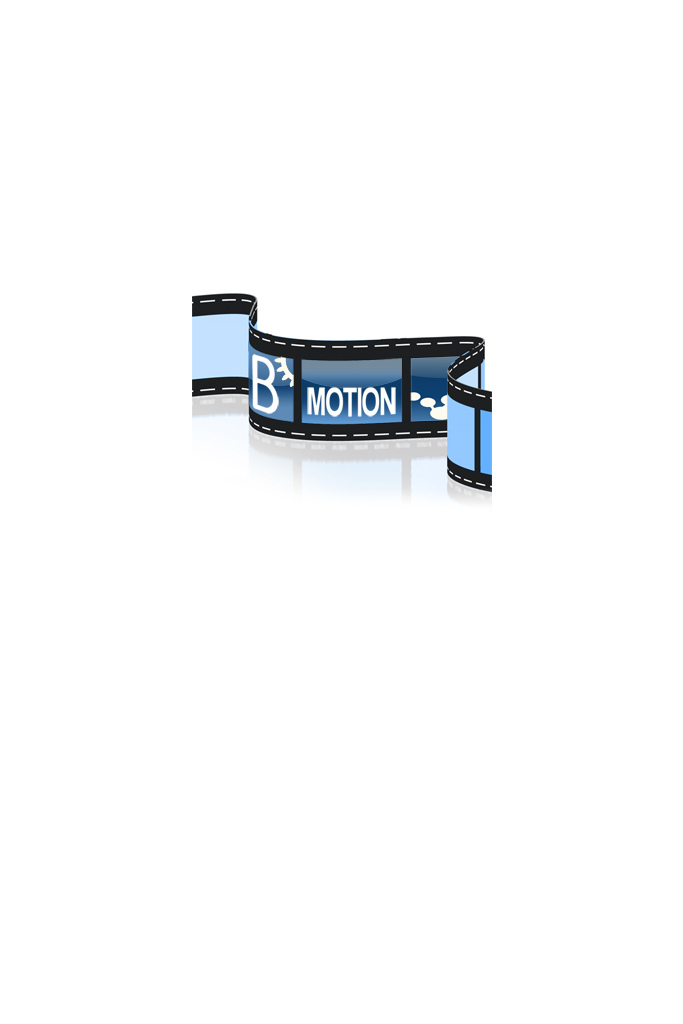
\includegraphics[width=\paperwidth,
keepaspectratio]{img/bms-handbook-bg.jpg}%
\vfill
}}}

\fi

%%% Local Variables: 
%%% mode: latex
%%% TeX-master: "rodin-doc"
%%% End: 


\title{BMotion Studio User's Handbook}
\author{
Work in Progress\\
Handbook $ $Rev: 16185 $ $ \\
\\
\href{mailto:ladenberger@cs.uni-duesseldorf.de}{ladenberger@cs.uni-duesseldorf.de}\\
\href{http://www.stups.hhu.de/ProB/index.php5/BMotion_Studio}{http://www.stups.hhu.de/ProB/index.php5/BMotion_Studio}
}

\begin{document}        
\pagestyle{empty}
\ifplastex
\maketitle
\else
\pagenumbering{roman}
\begin{titlepage}
\AddToShipoutPicture*{\BackgroundPic}
\vspace*{\titletop}
{\titledimrodin\selectfont \bfseries BMotion Studio}

\vspace*{\titlesubtitledistance}
{\titledimhandbook\selectfont \bfseries User's Handbook}

\vspace*{\titlesecdistance}
{\titledimsubtext\selectfont \textbf{\textsf{ProB Edition}}}

\vspace*{\titlesecdistance}
{\titledimsubtext\selectfont \textsf{Lukas Ladenberger (Editor)}}

\vspace*{\titlesecdistance}
{\titledimsponsor\selectfont %
  $\hbox{
\includegraphics[height=4ex]{img/advance-logo.png}}$
  \textsf{This work is sponsored by the ADVANCE Project}}

\vspace*{\titlebottom}

\end{titlepage}
\ifdefined\isinprint
\cleardoublepage
% Title page
\vspace*{10em}
\begin{center}
  {\huge \textbf{BMotion Studio User's Handbook}}\\
  \vspace{2em}
  {\large ProB Edition}
\end{center}
\clearpage
% Copyright page
\vspace*{\fill}
\noindent\textbf{BMotion Studio User's Handbook}\\
~\\
This work, except the cover image, is licensed under the Creative Commons Attribution-ShareAlike 3.0 Unported License. To view a copy of this license, visit \href{http://creativecommons.org/licenses/by-sa/3.0/}{creative\-com\-mons.org/\-licenses/\-by-sa/3.0/} or send a letter to Creative Commons, 444 Castro Street, Suite 900, Mountain View, California, 94041, USA.\\
The cover image of a Rodin statue was created by Miikka Skaffari.
It is licensed under a Creative Commons Attribution-NonCommercial 3.0 Unported License.  To view a copy of this license, visit \href{http://creativecommons.org/licenses/by-sa/3.0/}{creative\-com\-mons.org/\-licenses/\-by-sa/3.0/} or send a letter to Creative Commons, 444 Castro Street, Suite 900, Mountain View, California, 94041, USA.
\vspace{10em}
\else\fi
\cleardoublepage
\pagenumbering{arabic}
\phantomsection
\addcontentsline{toc}{chapter}{Contents}
\tableofcontents
\fi

\chapter{Introduction}
\label{introduction}

\section{Overview}

This handbook consists of five parts:

\begin{description}
	\item[Introduction (Chapter~\ref{introduction})] You are reading the introduction right now.  Its purpose is to help you orient yourself and to find information quickly.
	\item[Tutorial (Chapter~\ref{tutorial})] If you are completely new to BMotion Studio, the tutorial is a good way to get up to speed quickly.  It guides you through the installation and usage of the tool.
	\item[Reference (Chapter~\ref{reference})] The reference section provides comprehensive documentation of BMotion Studio and its components.
	\item[Frequently Asked Questions  (Chapter~\ref{faq})] Common issues are listed by category in the FAQ.
	\item[Index] We included an index particularly for the print version of the handbook, but it may be useful in the electronic versions as well.  
\end{description}

\subsection{Formats of this Handbook}
\label{handbook_formats}

The handbook comes in various formats:

\begin{description}
	\item[Online Help] You can access the handbook online at \url{http://www.stups.hhu.de/ProB/index.php5/BMotion_Studio}.
	\item[PDF Help] Both online versions also include a link to the PDF version of the handbook.
\end{description}

\section{Conventions}
\label{conventions}

We use the following conventions in this manual:

\tick{Checklists and milestones are designated with a tick. Here we summarize what we want to learn or should have learned so far.}
\info{Useful information and tricks are designated by the information sign.}
\warning{Potential problems and warnings are designated by a warning sign.}
\pencil{Examples and Code are designated by a pencil.}

We use \texttt{typewriter} font for file names and directories.

We use \textsf{sans serif font} for GUI elements like menus and buttons.  Menu actions are depicted by a chain of elements, separated by ``$\rangle$'', e.g. \textsf{File $\rangle$ New $\rangle$ Visualisation}.

\section{ADVANCE}
\label{advance}

This work has been sponsored by the Advance project\footnote{\url{http://www.advance-ict.eu/}}.  ADVANCE is an FP7 Information and Communication Technologies Project funded by the European Commission. The overall objective of ADVANCE is the development of a unified tool-based framework for automated formal verification and simulation-based validation of cyber-physical systems.

The ADVANCE project is unique in addressing both simulation and formal verification within a single design framework.

Unification is being achieved through the use of a common formal modelling language supported by methods and tools for simulation and formal verification. An integrated tool environment is providing support for construction, verification and simulation of models.

ADVANCE is building on an existing formal modelling language - Event-B - and its associated tools environment - Rodin - with strong support for formal verification. In ADVANCE, Rodin is being further strengthened and augmented with novel approaches to multi-simulation and testing.

\section{Creative Commons Legal Code}
\label{sec:cc}        

The work presented here is the result of an collaborative effort
that took many years.  To ensure that access to this work stays free
and to avoid any legal ambiguities, we decided to formally lincense
it under the Creative Commons Share-Alike License.

This work is licensed under the Creative Commons Attribution-ShareAlike 3.0 Unported License. To view a copy of this license, visit \url{http://creativecommons.org/licenses/by-sa/3.0/} or send a letter to Creative Commons, 444 Castro Street, Suite 900, Mountain View, California, 94041, USA.



% \section{Style Guide}
\label{style-guide}

\info{For now, we will manage the style guide as a \LaTeX~document together with the rest of the documentation.  We may take it out upon publication.}

\subsubsection{General Stylistic Guidelines}

\begin{itemize}
	\item The conventions (\ref{conventions}) are part of the style guide.

	\item Use the ``we'' form.

	\item We use British English.

	\item When referring to the different views in Rodin, the word ``view'' should be written in lowercase, e.g., the Rodin Problems view.
\end{itemize}

\subsubsection{Files}

Files should be saved in the \texttt{files} subdirectory. You can also create a subdirectory. Then, use the definition 

\begin{verbatim} \file{1}{2} 
\end{verbatim} 

to create a link to the file. The definition extends to arguments. The first argument (1) defines the file name i.e. \texttt{Celebrity.zip} or if you saved the file in a subdirectory \texttt{subdirectory/Celebrity.zip}. The second argument (2) defines the name which should be displayed in the document, i.e. ``Celebrity Problem Example Download''.

\warning{Please note, that you only enter the file name without a path before (expected subdirectories). The build script assigns the correct path to the file on the server automatically .}

Here is an example using the definition: \file{Celebrity.zip}{Celebrity Problem Example Download}.

\subsubsection{Avoiding Redundancy}

We will reduce (or avoid) redundancy through heavy linking, following these guidelines:

\begin{itemize}
	\item If in doubt, provide the bulk of the information in the Reference section.  For instance, the FAQ entry ``What is Event-B?''  Should simply refer to the Event-B entry in the Reference section.
	\item Web Links should not appear multiple times
	\item List web links as footnotes in the Tutorial and FAQ.
	\item List web links in a ``See also'' Section in the Reference.
\end{itemize}

\subsubsection{Sections}

\begin{itemize}
	\item If referring to a specific chapter or section, use uppercase to denote it, e.g. ``in Chapter~3''.
	\item We also refer to subsections as Section, e.g. ``see Section~2.5''
	\item We have a small number of well-defined chapters which are the top level structuring element.
	\item Sections and subsections are numbered.  In the HTML-Versions, they are broken into subpages.
    \item Subsubsections do not receive numbers and are not broken into subpages in the HTML.  Keep this in mind regarding both the reading flow and page sizes.
	\item Avoid linking (ref) to subsubsections, as they don't have a number.  Latex will instead provide a link to the next higher element.  This works, but it could create confusion.
	\item Generally, we should avoid gaps in the hierarchy (i.e. having a subsubsection in a section without a subsection in between).\footnote{Coincidentally, this style guide violates this rule. Reason: We want the style guide to remain whole and not be broken into subsections, but the proper hierarchy is a section.}
	\item Section labels should be all in lower case. Use ``\_'' for blanks.
	\item We use the prefix ``\texttt{int\_}'' for introduction section labels, ``\texttt{tut\_}'' for tutorial section labels following a meaningful description of the section (i.e. \texttt{tut\_rodin\_installation}) and ``\texttt{faq\_}'' for faq section labels following a short version of the title (i.e. \texttt{faq\_diff\_eventb\_b}). Reference section labels have no prefix.
\end{itemize}

\subsubsection{Images}
\begin{itemize}
	\item Images must be no more than 700 pixels in width (for HTML version) and no more than 160 mm (for PDF version). This is fairly easy for bitmaps (screenshot), pay attention to this regarding how plasTeX converts vector images. (see Latex section below on how to include images)

	\item Screenshots should look neat and consistent.  Horizontal real estate will always be an issue, so please resize the windows before taking the screenshot to keep things readable at 700 pixel width.  (see Latex section below on how to include images)

	\item Images should always have a caption and a label. Please use the same conventions for the figure labels that are used for the the section labels, but use the prefix ``\texttt{fig\_}''. \\Example: ``\texttt{fig\_tut\_03\_traffic\_light}''. For referencing do not use references like "As shown bellow" or "Like in the following image:". Use always a format like:

\begin{verbatim}"... as shown in figure \ref{fig_tut_03_traffic_light}."\end{verbatim}

	\item We use icons from Pixel-Mixer, which are free as long as credit is given: \url{http://www.softicons.com/free-icons/toolbar-icons/basic-icons-by-pixelmixer}

  \item We include Window decoration only when it is really necessary.  If we discuss only some views, we crop the rest away.  Please crop neatly, following edges. Even if you need a screenshot with window decoration, you should always use the same Window decoration (i.e. linux ubuntu default decoration style). If you need such a screenshot, please contact Lukas.

  \item Image file names should be all in lower case and not include umlaute or special characters. Use ``\_'' for blanks.

  \item Image files should keep the following rules:
	
\begin{itemize}
		\item Tutorial images should be saved in the sub folder \texttt{img/tutorial} with the prefix ``\texttt{tut\_}'' following the section number. For instance, \texttt{tut\_01\_image1.png}.

		\item FAQ images should be saved in the sub folder \texttt{img/faq} with the prefix ``\texttt{faq\_}''. For instance, \texttt{faq\_image1.png}.

	\end{itemize} 
	\end{itemize}

\subsubsection{Icons}

For icons (i.e. RODIN platform icons) in continuous text use the command: 

\begin{verbatim} \icon{1} \end{verbatim} 

The first (1) argument takes the path to the icon (i.e. \texttt{rodin/auto\_prover.png}). You can find all icons in the folder \texttt{latex/img/icons/}

Here is an example using icons in continuous text:

\textit{Lorem ipsum dolor sit amet, consetetur \icon{rodin/auto_prover.png} sadipscing elitr, sed diam nonumy eirmod tempor invidunt ut labore et dolore magna aliquyam erat, sed diam voluptua. At vero eos et accusam et justo duo dolores et ea rebum. Stet clita kasd gubergren, no sea takimata sanctus est Lorem ipsum dolor sit amet. Lorem ipsum dolor sit amet, consetetur sadipscing elitr, sed diam nonumy eirmod tempor invidunt ut labore et dolore \icon{rodin/lasoo_prover.png} magna aliquyam erat, sed diam voluptua. At vero eos et accusam et justo duo dolores et ea rebum. Stet clita kasd gubergren, no sea takimata sanctus est Lorem ipsum dolor sit amet.}

\subsubsection{Index}
Please add meaningful entries to the index. This helps users to look up information more efficiently.
The \LaTeX-command to do this is \verb#\index{#\textit{word}\verb#}#.
\begin{itemize}
\item The most important thing to think about when considering the index is the user perspective: 
  What is the word that a user will look up to try and find this topic?
\item An index entry should be a noun, singular and written in lowercase (uppercase if it's a name).
\item If the word appears in are several locations in the documentation (e.g. in the tutorial and the
  reference section), try to highlight the most commonly used location with \verb#\index{word|textbf}#.
  This is usually an entry in the reference section.
\item Adjectives should be used with care. 
  Please use them only if omitting the adjective changes the meaning of the entry drastically or
  if the adjective is necessary to distinguish the entry from other entries with the same noun but
  other location.
\item If you use an adjective, consider using the noun as a key for sorting: \verb#\index{cloud,grey@grey cloud}#
  instead of \verb#\index{grey cloud}#
\item If you have multiple entries for the same word, consider using sub-entries (\verb#\index{cloud!grey}#)
  if different things are meant. Another example is \verb#\index{true!as predicate}# and \\ \verb#\index{true!as expression}#
\item Multiple index entries for the same text block are alright.
\item If you use the index command, please have a look at the result.
\end{itemize}

\subsubsection{\LaTeX{} Styling}

\begin{itemize}
	\item Try to avoid fancy \LaTeX formatting, as PlasTeX (used for generating HTML) is temperamental.  Macros are especially problematic, and sometimes the result is just ugly.
	\item We have the option to use different files to generate the PDF and HTML, but we would generally prefer not to do this.  Look at \texttt{bsymb.sty} and \texttt{plastex-bsymb.sty} as an example. \textbf{NOTE:} We don't do this any more for any style files.
	\item Every section should have a label, reflecting the section name, all lowercase, spaces replaced with underscores (\_).
	\item Don't create subdirectories in the \texttt{latex} folder, as the scripts cannot always deal with them.
	\item Put images in the \texttt{img} folder.  Feel free to create additional directory structures underneath.
	\item Files other than images (e.g. Event-B projects) --- we have macros to link them absolute in the PDF, and to link them relative in HTML and Eclipse Help.
	\item Use linked sections numbers (generated with \texttt{\\ref{}} instead of hyperlinks for cross-references. This is necessary for the print documentation to be useful.
	\item When including images in Latex, do not provide a width!  Instead, try to embed the print size in the image itself.  For instance, PNGs allow you to set the print size (in mm).  This way we can be sure that the images are rendered as HTML without distortion.
\end{itemize}

\subsubsection{Contributions from Plugin Developers}
\label{sec:plugin_contributions}

\begin{rodin-plugin}{prob.png}{ProB}
We want to encourage Plugin developers to contribute to the Handbook, but we have to make it clear that we cannot maintain that documentation.  Therefore, it has to be clearly marked.  We use a custom environment for that purpose that
(1) provides the Plugin's icon, (2) adds a disclaimer to the end of the custom documentation and (3) puts the content into a gray box (like this one).

There are some limitations to the environment that we use.  Specifically, headlines and images should be kept outside the gray box.

\end{rodin-plugin}

%%% Local Variables: 
%%% mode: latex
%%% TeX-master: "rodin-doc"
%%% End: 


\section{Background}

\subsection{BMotion Studio}

\begin{figure}[!ht]
\begin{center}
	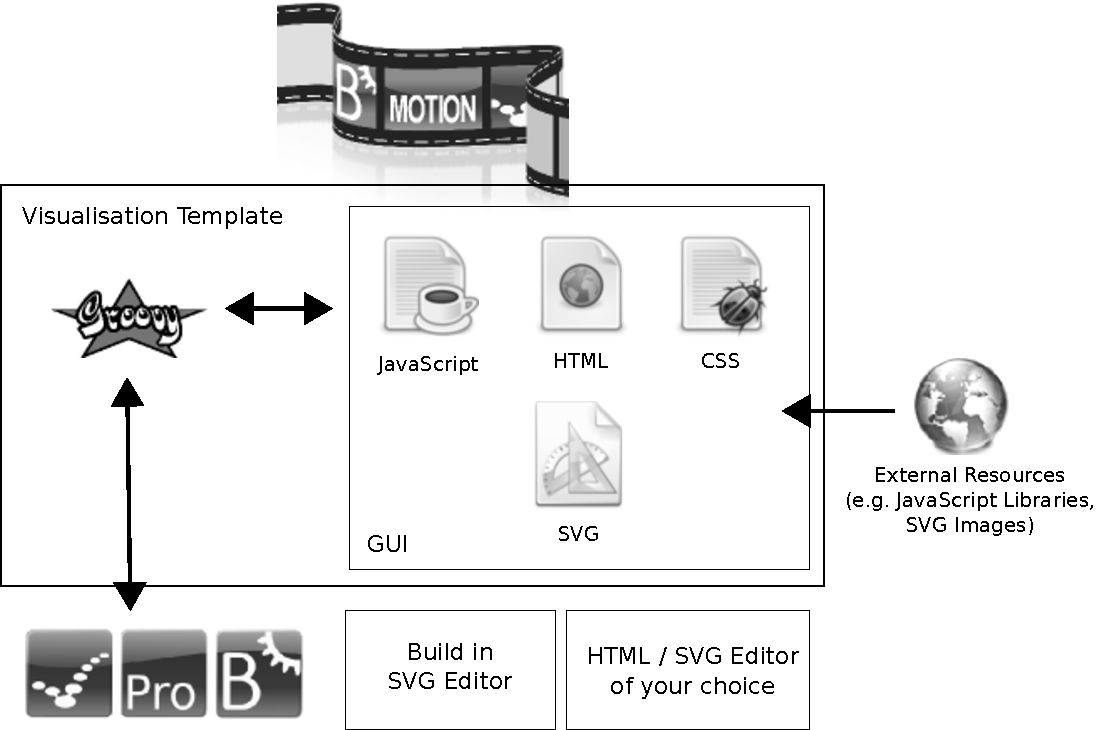
\includegraphics[width=14cm]{img/tutorial/bms_architecture}
	\caption{\bms~Architecture}
	\label{fig_tut_00_architecture}
\end{center}
\end{figure}

Figure~\ref{fig_tut_00_architecture} shows an overview of the architecture of \bms. 
In \bms, a visualisation is described by a visualisation template that contains visual elements and observers. 
Visual elements may be, for instance, shapes or images that represent some aspects of the model. 
For example, when modelling a communication protocol, circles may be used for representing the communicating entities of the protocol and arrows for the message exchanges between the entities. 
\bms~supports web technologies like Scalable Vector Graphics (SVG)\footnote{\url{http://www.w3.org/TR/SVG11}} and Cascading Style Sheets (CSS)\footnote{\url{http://www.w3.org/TR/css-2010}} for this purpose. 
SVG is an XML-based markup language for describing two-dimensional vector graphics. 
It comes with a number of visual elements like shapes, images and paths.
CSS is a language that can be used to describe the style of SVG visual elements (e.g. the colour or the dimension). 

Observers are used to link visual elements with the model. 
An observer is notified whenever a model has changed its state, i.e. whenever an event has been executed. 
In response, the observer will query the model's state and triggers actions on the linked visual elements in respect to the new state. 

\subsection{Formal Modelling}

We are concerned with \textit{formalizing specifications}.  This allows us a more rigorous analysis (thereby improving the quality) and allows the reuse of the specification to develop an implementation.  This comes at the cost of higher up-front investments.

This differs from the traditional development process. In a formal development, we transfer some effort from the test phase (where the implementation is verified) to the specification phase (where the specification in relation to the requirements is verified).

\subsection{Predicate Logic}
\label{predicate_logic}
\index{predicate logic}

Predicate logic is a mathematical logic containing variables that can be quantified.

Event-B supports first-order logic which is, technically speaking, just one type of predicate logic.  

\subsection{Event-B}
\label{eventb}
\index{Event-B}

Event-B is a notation for formal modelling based around an abstract machine notation (\index{abstract machine notation}).

Event-B is considered an evolution of B (also known as Classical B). It is a simpler notation which is easier to learn and use. It comes with tool support in the form of the Rodin Platform.

\subsection{Classical-B}
\label{classicalb}
\index{Classical-B}

\subsection{CSP}
\label{csp}
\index{CSP}

\subsection{ProB Animator}
\label{prob_animator}

ProB is a validation toolset for the B method including an animator, a modelchecker and other useful tools to allow users to gain confidence in their specifications. One of the components of ProB is animation. The animation component allows the user to check the presence of desired functionality and to inspect the behaviour of a specification by "clicking through" the states of the specification. ProB also provides other useful tools such as a tool to visualize graphically any predicate as a tree or a tool for graphical state representation. Such tools, especially the tool for the graphical state representation can give a better understanding of the model.

\section{First Steps}
\label{first_steps}

\subsection{Installation}
\label{installation}

Start off by downloading \bms~for your operating system. 
You can find the latest version of the tool at \url{http://www.stups.hhu.de/ProB/index.php5/BMotion_Studio}.
Decompress the archive and expand the directory if necessary. 

%\warning{Do not change the location and structure of the files and directories within the folder!}

Navigate to the \texttt{bin} folder and start the tool by entering the bash command:

\begin{lstlisting}[language=bash]
.\bmotion-prob
\end{lstlisting}

\info{Windows users should execute the \texttt{bmotion-prob.bat} file.}

That's all! 
Your default browser should open and show the default workspace.
The workspace contains the following predefined folders:

\begin{itemize}
\item \texttt{lib}: This folder contains JavaScript libraries that are needed for BMotion Studio.
\item \texttt{b\_template}: A visualisation template for creating visualisations for Classical-B and Event-B models.
\item \texttt{csp\_template}: A visualisation template for creating visualisations for CSP models.
\end{itemize}

\subsection{Creating a new Visualisation Template}
\label{vis_template}

%Let's start by creating a new visualisation template.
The easiest way to create a new visualisation template is to duplicate one of the default templates  \texttt{b\_template} (for Event-B or Classical-B visualisations) or \texttt{csp\_template} (for CSP-M visualisations) that are included in the \texttt{workspace} folder of your \bms~installation.
Just duplicate the folder.
After refreshing your browser, the newly created folder should appear in your workspace.
Navigate to the folder. 
The folder contains three files:
\begin{itemize}
\item \texttt{template.html}: The HTML file is the root file of your visualisation. It contains the actual visualisation and it's configuration.
\item \texttt{template.groovy}: The Groovy script file is the place where the user can communicate with the formal model by means of the ProB Java API\footnote{\url{http://www.stups.hhu.de/ProB/index.php5/ProB_Java_API}}.
For instance, the user may register methods that can be called in the JavaScript file.
%The Groovy script file is the place where you can setup the communication between your visualisation and the ProB animator.
%In particular, the Groovy script file is the link between the formal model and the visualisation.
%It allows you to programmatically control the ProB animator and to access the actual formal model being visualised.
%In addition, you can register functions that can be called from the visualisation, e.g. executing an Event-B event after pressing a button in the visualisation.
\item \texttt{template.js}: In the JavaScript file you can setup observers and actions.
Moreover, the user can take advantage of the entire JavaScript language.
There exist are a lot of libraries for JavaScript that you can apply to create custom visualisations.
For instance, it exists libraries for manipulating the DOM of an HTML document, or for generating chart and plot diagrams.
%In addition, you can call functions that are registered in the Groovy script file.
%This enables you to add some interactivity to your visualisation.
%For instance, pressing a button in your visualisation could cause the execution of an Event-B event.
\end{itemize}

Here is an example HTML file:

\begin{lstlisting}[language=html]
<html bms-app>
  <head>
      <title>BMotion Studio for ProB</title>
      <meta name="bms.tool" content="BAnimation" />
      <meta name="bms.script" content="template.groovy" />
      <script src="/bms/libs/requirejs/require.js"></script>
      <script>
        require(['/bms/libs/prob/config.js'], function () {
          require(['template']);
        });
      </script>
  </head>
  <body>
  </body>
</html>
\end{lstlisting}

The meta tag \textit{bms.tool} (line 4) defines the formalism or the simulator respectively that should be used. 
Two values are allowed: ``BAnimation'' for creating visualisations of Event-B or Classical-B models and ``CSPAnimation'' for creating visualisations of CSP-M models.
The meta tag \textit{bms.script} (line 5) contains the link to the Groovy script file.
Finally, in line 9 we define the path to the JavaScript file.

\subsection{Linking a Model with the Visualisation}

In order to link a model with a visualisation, open the HTML file with an HTML/text editor of your choice and add the following line within the head tag, where XXX is the relative path to your model file (e.g. ``model/my-model.mch''):

\begin{lstlisting}[language=html]
<meta name="bms.model" content="XXX" />
\end{lstlisting}

Linking a model within the html file automatically loads the model, when starting the visualisation.

\subsection{Creating a Visualisation}
\label{create_vis}

The user is not restricted to an editor in order to create a visualisation.
The user can make use of any tool that support the creation of SVG graphics or HTML documents.
For the tutorials (Section~\ref{tutorial_b} and~\ref{tutorial_csp}) we are going to use the Inkspace\footnote{\url{https://inkscape.org}} editor. Inkscape is an editor for creating vector graphics that is available for Windows, Mac OS X and Linux.
It's free and open source.
With Inkscape the user can export the vector graphic into the SVG format.

\begin{figure}[!ht]
\begin{center}
	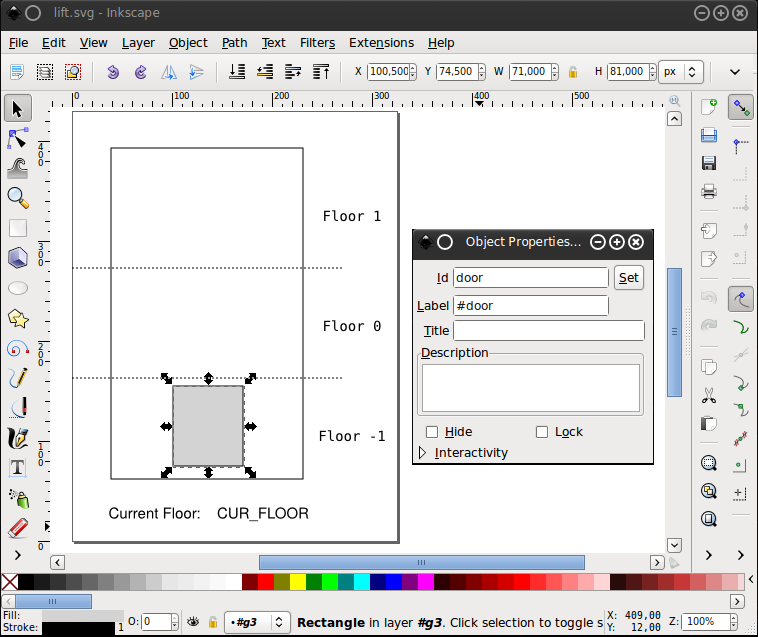
\includegraphics[width=12cm]{img/tutorial/tut_02.png}
	\caption{Creating an SVG graphic with Inkscape}
	\label{fig_tut_02_inkscape}
\end{center}
\end{figure}

\chapter{BMotion Studio for Event-B and Classical-B}
\label{bms4b}

\section{Tutorial}
\label{tutorial_b}

The objective of this chapter is to get you to a stage where you can use BMotion Studio to visualize Event-B or Classical-B models. 
We expect that you have already downloaded the BMotion Studio tool (see Section~\ref{installation}).
 
%We expect you to have a basic understanding of logic and an idea why doing formal modelling is a good idea.  
You should be able to work through the tutorial with no or little outside help.
We encourage you not to download solutions to the examples but instead to actively build them up yourself as the tutorial progresses.
If something is unclear, remember to check the Reference (\ref{reference_b}) for more information.

\subsection{Preparation}

Let's start by creating a new visualization template as described in Section~\ref{vis_template}.
Just download the \file{bms-b-template.zip}{predefined template}, decompress the archive and rename the folder to \texttt{lift}.
%After refreshing your browser, a new folder called \texttt{lift} should appear in your workspace (see Figure~\ref{fig_tut_01_workspace}).

%\subsection{Creating a new visualization Template}
%
%Let's start by creating a new visualization template.
%The easiest way to create a new visualization template is to duplicate the default template \texttt{b\_template} that is included in the \texttt{workspace} folder of your \bms~installation.
%Just duplicate the \texttt{b\_template} folder and rename it to \texttt{lift}.
%After refreshing your browser, a new folder called \texttt{lift} should appear in your workspace (see Figure~\ref{fig_tut_01_workspace}).
%Navigate to the \texttt{lift} folder. 
%The folder contains three files:
%\begin{itemize}
%\item \texttt{template.html}: The HTML file is the root file of your visualization. It contains the actual visualization and it's configuration.
%\item \texttt{template.groovy}: The Groovy script file is the place where the user can communicate with the formal model by means of the ProB Java API\footnote{\url{http://www.stups.hhu.de/ProB/index.php5/ProB_Java_API}}.
%For instance, the user may register methods that can be called in the JavaScript file.
%%The Groovy script file is the place where you can setup the communication between your visualization and the ProB animator.
%%In particular, the Groovy script file is the link between the formal model and the visualization.
%%It allows you to programmatically control the ProB animator and to access the actual formal model being visualised.
%%In addition, you can register functions that can be called from the visualization, e.g. executing an Event-B event after pressing a button in the visualization.
%\item \texttt{template.js}: In the JavaScript file you can setup observers and actions.
%Moreover, the user can take advantage of the entire JavaScript language.
%There exist are a lot of libraries for JavaScript that you can apply to create custom visualizations.
%For instance, it exists libraries for manipulating the DOM of an HTML document, or for generating chart and plot diagrams.
%%In addition, you can call functions that are registered in the Groovy script file.
%%This enables you to add some interactivity to your visualization.
%%For instance, pressing a button in your visualization could cause the execution of an Event-B event.
%\end{itemize}
%
%\begin{figure}[!ht]
%\begin{center}
%	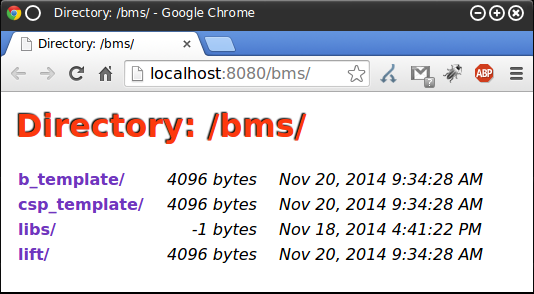
\includegraphics[width=12cm]{img/tutorial/tut_01.png}
%	\caption{\bms~Workspace}
%	\label{fig_tut_01_workspace}
%\end{center}
%\end{figure}

\subsection{The Formal Model}

We are going to create a visualization	for a simple lift system that allows movement of a single lift cage between three floors.
The door of the lift can be closed and opened - all in response to the pressing of floor call and cage send buttons.

You can download the Event-B model \file{EventBLift.zip}{here}.
Decompress the archive and put the files into a new folder called \texttt{model} relative to your \texttt{index.html} file.

\subsection{Link the Model with the Visualization}

The first step consists of linking the model with the visualization.
For this, open the \texttt{bmotion.json} file with an editor of your choice and set the \textit{model} path property to ``model/MLift.bcm''.
This links the visualization with the Event-B machine called ``MLift''.
Linking a model within the \texttt{bmotion.json} file will automatically load the model, when starting the visualization (see Section~\ref{sec:stat_vis}).

\subsection{Create the Actual Visualization}

Please download the prepared \file{lift.svg}{lift.svg} file and open it with Inkscape as demonstrated in Figure~\ref{fig_tut_02_inkscape}.
Feel free to modify and explore the SVG graphic.
In order to link graphical elements of the SVG graphic with the formal model later, we have to give them identifiers. 
For this, select an element in Inkscape, open the context menu and select \textsf{Object Properties}.
A popup window should be opened as demonstrated in Figure~\ref{fig_tut_02_inkscape}.
As an example, we give the graphical element that represents the door (the gray filled rectangle), the id ``door''.
In Section~\ref{sec_creation_observers} we explain how we can use this information in order to establish \textit{observers}.
If you are satisfied with your SVG graphic, save it as a plain SVG graphic with \textsf{File $\rangle$ Save As}.
Select \textsf{Plain SVG (*.svg)} as an output format and click on the \textsf{Save} button.
You can save the SVG file anywhere on your local system. 
Open the SVG file with an editor of your choice, copy the SVG code and paste it within the body tag in the \texttt{index.html} file.

\subsection{Start the Visualization}
\label{sec:stat_vis}

Let's try out the visualization for the first time!
Just drag and drop the \texttt{bmotion.json} file on the marked area or open it via the file dialog.
%In your browser, navigate to the folder \texttt{lift} folder and click on the \texttt{template.html} file.
The visualization should start.
At the right bottom you will find a menu called \textsf{Open View} for opening different ProB related views.
For instance, Figure~\ref{fig_tut_03_running1} shows the running lift visualization with the ProB Events view opened.

At the moment nothing spectacular happens when changing the state (i.e. executing events in the Event view), because no observers were created.
In the next Section we learn how we can link graphical elements with the formal model by establishing observers.

\begin{figure}[!ht]
\begin{center}
	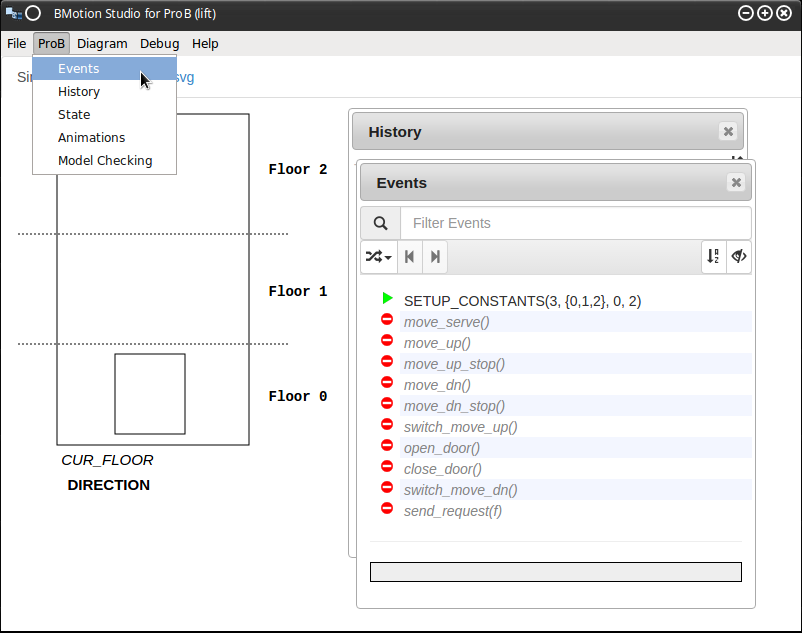
\includegraphics[width=12cm]{img/tutorial/tut_03.png}
	\caption{Running the Lift visualization for the First Time}
	\label{fig_tut_03_running1}
\end{center}
\end{figure}

\subsection{Create Observers}
\label{sec_creation_observers}

Observers are used to link graphical elements with the model. 
An observer is notified whenever the model has changed its state, i.e. whenever an event has been executed. 
In response, the observer will query the model's state and triggers actions on the linked graphical elements in respect to the new state.
Observers are written in JavaScript and should be placed in the \texttt{script.js} file.
As an example, consider the following observer:

\begin{lstlisting}[language=JavaScript, caption={Formula Observer Displaying the Current Floor (JavaScript)}]
$("#txt_cur_floor").observe("formula", {
  formulas: ["cur_floor"],
  trigger: function (origin, result) {
    origin.text(result[0])
  }
});
\end{lstlisting}

We are going to explain the JavaScript code line by line.
In line 1 we register a formula observer on the graphical element with the id \textit{txt\_cur\_floor} that is located in our \texttt{index.html} file.
%Line 1 means that we want to transform the graphical element with the id \textit{txt\_cur\_floor} that is located in our \texttt{index.html} file.
\bms~follows the jQuery selector syntax\footnote{\url{http://api.jquery.com/category/selectors}} to select elements.
The prefix ``\#'' denotes that we want to select an element by its id.
In line 2 we define a list of observed formulas.
In this case we observe the variable \textit{cur\_floor}.
In line 3 to 5 we define a trigger function that is called after every state change with its \textit{origin} (the origin parameter holds a reference to the element that the observer is attached to\footnote{Checkout the jQuery API for more information \url{https://api.jquery.com}.}) and the \textit{result} (the result parameter contains the results of the defined formulas in an array, e.g. use \textit{result[0]} to obtain the result of the first formula).
The trigger function changes the text of the graphical element (\textit{origin}) to the current value of the variable \textit{cur\_floor} (\textit{result[0]}).
%Reload the visualization by clicking on the \texttt{Reload} button and play with the visualization by executing some events.
%Line 2 affects that the attribute \textit{text} will be set to the value that is returned by the followed closure.
%In particular, the closure evaluates the expression \textit{cur\_floor} in the current state and returns the value to be set.
%In other words, the observer sets the current value of the variable \textit{cur\_floor} into the visual text element with the id \textit{txt\_cur\_floor}.
%Line 3 is responsible to register the observer.
%All registered observer will be triggered after every state change.

Let's create another observer.
Check out the following code:

\begin{lstlisting}[language=JavaScript, caption={Formula Observer for the Lift Door (JavaScript)}]
$("#door").observe("formula", {
  formulas: ["cur_floor", "door_open"],
  trigger: function (origin, result) {
    
    switch (result[0]) {
      case "0":
        origin.attr("y", "175");
        break;
      case "1":
        origin.attr("y", "60");
        break;
      case "-1":
        origin.attr("y", "275");
        break;
    }
    
    if(result[1] === "TRUE") {
      origin.attr("fill", "white");
    } else {
      origin.attr("fill", "lightgray");
    }
    
  }
});
\end{lstlisting}

In line 1 we register a formula observer on the graphical element with the id \textit{door}, similar to the previous defined observer.
%Line 1 means that we want to transform the graphical element with the id \textit{door}, similar to the previous observer.
In line 2 we define the set of observed formulas (\textit{cur\_floor} and \textit{door\_open}).
In line 3 to 23 we define a trigger function, that makes the following action:
Line 5 to 15 will switch the \textit{y} coordinate of the door (denoting the movement of the door between floors) according to the current value of the variable \textit{cur\_floor} (\textit{result[0]}).
Lines 17 to 21 affect that the attribute \textit{fill} of the door will be set to ``white'' (denoting the door is open) whenever the formula \textit{door\_open} evaluates to \textit{TRUE} in the current state (\textit{result[1]}), otherwise to ``lightgray'' (denoting the door is closed).
%Whenever the expression \textit{door\_open} evaluates to \textit{TRUE}, the value \textit{white} (denoting the door is opened) is returned, otherwise the value \textit{lightgray} (denoting the door is closed) is returned.
%Line 3 to 17 will switch the \textit{y} coordinate of the door (denoting the movement of the door between floors) according to the evaluation result of the expression \textit{cur\_floor}.
%In line 18 we register the observer.
%You can use the entire Groovy power and feature range for defining your observers.

Add both snippets to your \texttt{script.js} file and click on the \texttt{Reload} button.
Let's see how this affects the visualization:
Setup and initialize the machine using the ProB events view.
Execute some events and see what happens.
For instance, Figure~\ref{fig_tut_04_running2} shows the lift visualization where the lift is on floor 0 and the door is open.

\begin{figure}[!ht]
\begin{center}
	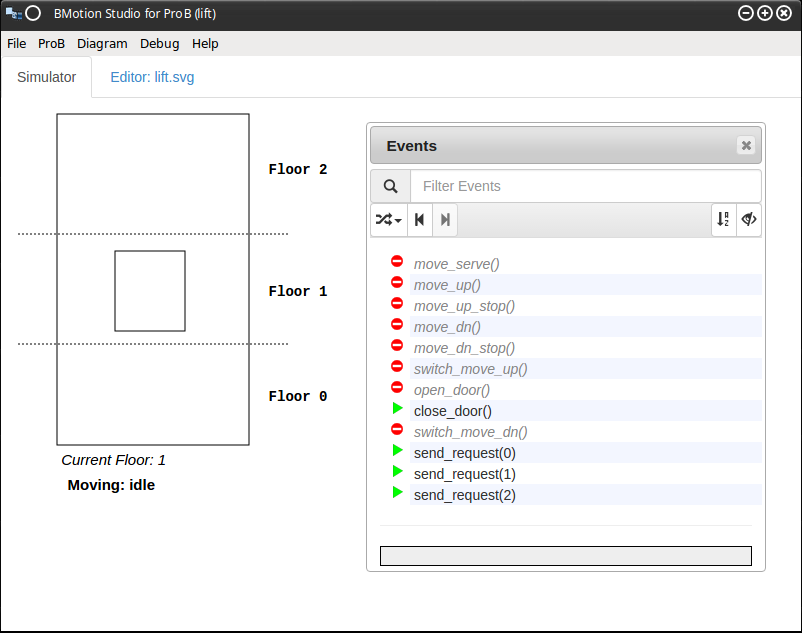
\includegraphics[width=12cm]{img/tutorial/tut_04.png}
	\caption{Lift visualization with observers}
	\label{fig_tut_04_running2}
\end{center}
\end{figure}

\subsection{Add Event Handler}

In this Section we learn how we can enhance our visualization with interactive features, e.g. executing an Event-B event by clicking on a graphical element.

Let's add an interactive feature, where the user can click on a floor label to order the lift on the corresponding floor.
Add this code snippet to your \texttt{script.js} file:
\newpage
\begin{lstlisting}[language=JavaScript, caption={Example of an Interactive Feature (JavaScript)}]
$("text[data-floor]").executeEvent({
  events: [
    {
      name: "push_call_button", 
      predicate: function (origin) {
        return "b=" + $(origin).attr("data-floor")
      }
    }
  ]
});
\end{lstlisting}

%For instance, clicking on the floor Label ``Floor 1'' should execute the Event-B event \textit{push\_call\_button(1)}.
In line 1 we register an execute event handler for each graphical element that matches the defined selector ``text[data-floor]''.
In particular, the selector matches the three floor labels (see Figure~\ref{fig_tut_03_running1}).
In line 2 to 9 we define the list of events that should be wired with the graphical elements.
Every event should contain the \textit{name}.
In addition, the user may enter a \textit{predicate} that defines the event's arguments.
If the user defines more than one event, a tooltip will be shown with a list of the defined events after clicking on the graphical element.
In our example we define only one event with the \textit{name} $push\_call\_button$ and the \textit{predicate} that is determined by a closure that passes a reference to the element (\textit{origin}).
In particular, we use the value of the attribute \textit{data-floor} of the corresponding floor label (\textit{origin}) to define the event parameter (line 6).

Apply these changes by clicking on the \texttt{Reload} button and try to click on a floor label.
This should call the Event-B event \textit{push\_call\_button} with the corresponding predicate/parameter.

Let's add another interactive feature, where the user can click on the graphical element that represents the door to open or close the door respectively.
%The first step consists of registering a new Groovy function that executes the corresponding event \textit{open\_door} or \textit{close\_door}.
%Add the code snippet to your \texttt{template.groovy} file:
%\begin{lstlisting}[language=Groovy, caption={Registering a Groovy Function (Groovy)}]
%bms.registerMethod("openCloseDoor", {
%    def Trace t = bms.getTool().getTrace()
%    def Trace newTrace = executeEvent(t, "open_door", []) ?: executeEvent(t, "close_door", [])
%    if (newTrace != null) {
%        animations.traceChange(newTrace)
%        return [newState: newTrace.getCurrentState().id]
%    }
%})
%
%def Trace executeEvent(t,name,pred) {
%    try {
%        t.execute(name, pred)
%    } catch(IllegalArgumentException e) {
%        null
%    }
%}
%\end{lstlisting}
%In Line 1 we register a new Groovy function called \textit{openCloseDoor}.
%The next lines show an example how we can use the ProB Java API.
%In Line 2 we get the current trace of the animation.
%In Line 3, we first try to execute the \textit{open\_door} event by means of a helper method called \textit{executeEvent} (Line 10 to 16).
%If the return value of the helper method is null (the event could not be executed), we try to execute the event \textit{close\_door}.
%If we success (we executed one of the both events), we trigger a trace change, causing to refresh the current animation (Line 5).
%This in turn changes the state and triggers our registered observers.
%Line 6 returns a Json object that contains the state id of the new state.
%This information can used later at the JavaScript side after executing the registered \textit{openCloseDoor} method.
%Let's switch to the JavaScript side.
Add the following code snippet to your \texttt{script.js} file:
%\begin{lstlisting}[language=JavaScript, caption={Call openCloseDoor Groovy Method (JavaScript)}]
%$("#door").click(function () {
%	bms.callMethod("openCloseDoor", {
%		callback: function (data) {
%			console.log("Callback: " + data)
%		}
%	})
%}).css("cursor", "pointer")
%\end{lstlisting}
\begin{lstlisting}[language=JavaScript, caption={Interaction with the Lift Door (JavaScript)}]
$("#door").executeEvent({
  events: [
    { name: "close_door" }, 
    { name: "open_door" }
  ]
});
\end{lstlisting}

In line 1 we register a new execute event handler on the graphical element with the id door.
The execute event handler first tries to execute the event \textit{close\_door}.
In case the event is disabled, it tries to execute the next event \textit{open\_door}.
%Line 2 calls our registered Groovy method \textit{openCloseDoor}.
%In Line 3 to 5 we pass a callback function that is called after an event (\textit{open\_door} or \textit{close\_door}) was executed.
%In this case we print the returned new state id on the console.

These are only small examples for adding interactivity to your visualization.
You are not limited to these examples.

\subsection{Final visualization}

You can download the final visualization \file{LiftVisualisation.zip}{here}.

\section{Reference}
\label{reference_b}

%\subsection{Observers}
%\label{sec:observers}
%
%Observers are used to link visual elements with the model. 
%An observer is notified whenever a model has changed its state, i.e. whenever an event has been executed. 
%In response, the observer will query the model's state and triggers actions on the linked graphical elements in respect to the new state. 
%
%\subsection{Observers in Groovy}
%\label{sec:groovy_observers}

%In general, observers are defined in the Groovy script file.
%\bms~comes with some predefined observers that are described in the following sections.

%\subsubsection{Transformer Observer}
%\label{sec:transformer_observer}

%The transformer observer supports the modification of attributes of graphical elements based on the %current state of the animation.
%The following code snippet demonstrates the basic use of the transformer observer:

%\begin{lstlisting}[float=ht,language=Groovy]
%transform("#myvisualelement") {
%    set "fill", "green"
%    set "stroke", "red"
%    register(bms)
%}
%\end{lstlisting}

%In line 1 we define a jQuery selector to select the graphical elements which should be transformed.
%In this case we select a visual element with the id \textit{myvisualelement} (in jQuery the prefix %``\#'' denotes that we want to select and element by its id).
%jQuery provides several possibilities to select graphical elements.

%\info{The jQuery selector API documentation\footnote{\url{http://api.jquery.com/category/selectors/}} provides an overview and a detailed documentation about selectors.}

%Line 2 to 3 are actions that are made on the graphical elements which are matched by the defined selector.
%In this case the \textit{fill} attribute is set to the value \textit{green} and the \textit{stroke} attribute to \textit{red}.
%In line 4, we register the observer to the current visualisation.
%A registered observer is triggered after every state change, e.g. after executing an event.
%
%\paragraph{Groovy Closures.}
%%As we use the Groovy Scripting language for defining the observers, we can make use of the entire function and feature range of it.
%Transformer observers support the use of Groovy closures for defining the selector or the value of an action.
%The following code snippet demonstrates the use of closures for transformer observers:
%
%\begin{lstlisting}[float=ht,language=Groovy]
%transform("#myvisualelement") {
%  set "fill", { (bms.eval("1 < x").value == "TRUE") ? "white" : "lightgray" }
%  set "y", {
%    switch (bms.eval("x").value) {
%      case "0": "15"
%        break
%      case "1": "20"
%        break
%      case "2": "25"
%        break
%      default: "0"
%    }
%  }
%  register(bms)
%}
%\end{lstlisting}
%
%In Groovy a closure is encapsulated in curly brackets.
%Line 2 and 3 show two examples for using closures for defining the value of the attribute \textit{fill} and \textit{y} respectively.
%Closures are evaluated after every state change in consequence of triggering the transformer observer.
%As an example, in line 2 the closure evaluates the expression $1 < x$.
%The value of the \textit{fill} attribute is set to \textit{white} whenever the expression evaluates to \textit{TRUE} and otherwise to \textit{lightgray}.
%
%
%\subsubsection{Method Observer}
%\label{sec:method_observer}
%
%The following code snippet gives an example of the method observer:
%
%\begin{lstlisting}[float=ht,language=Groovy]
%callMethod("mymethod") {
%  data([foo: "bar"])
%  register(bms)
%}
%\end{lstlisting}
%
%\subsubsection{Custom Observer}
%\label{sec:custom_observers}
%
%The following code snippet gives an example of a custom observer:
%\begin{lstlisting}[float=ht,language=Groovy]
%def customObserver = [ 
%  apply: { bms ->  println "Triggering custom observer." } 
%] as BMotionObserver
%bms.registerObserver(customObserver)
%\end{lstlisting}
%
%You can also create a custom transformer observer:
%\begin{lstlisting}[float=ht,language=Groovy]
%def transformerObserver = [
%  update: { bms ->
%    def transformers = []
%    def result = bms.translate("relation")					
%    result.value.each { obj ->
%      transformers += transform("#" + obj.first) {
%        set "transform", "translate(" + obj.second + ")"
%        update(bms)
%      }
%    }
%    return transformers
%  }
%] as BMotionTransformer
%bms.registerObserver(transformerObserver)
%\end{lstlisting}

\subsection{Observers}
\label{b_observers}

Observers are used to link graphical elements with the model. 
An observer is notified whenever a model has changed its state, i.e. whenever an event has been executed. 
In response, the observer will query the model's state and triggers actions on the linked graphical elements in respect to the new state. 

In general, observers are defined in the JavaScript file. 
\bms~comes with some predefined observers that are described in the following sections.

\subsubsection{Formula Observer}

The formula observer \textit{observes} a list of formulas (i.e. expressions, predicates or single variables) and triggers a function whenever a state change occurred.
The result of the formulas are passed to the trigger function.
For instance, the trigger function can change the attributes of the graphical elements (e.g. the colour or position) according to the results of the formulas in the respective state.
The following options can be passed to the formula observer:

\begin{itemize}

	\item[] \textbf{selector [Type: string]:}\\ A \textit{selector} that matches a set of graphical elements in the visualization (e.g. images or shapes). 
A selector follows the syntax provided by jQuery\footnote{For more information about jQuery and selectors we refer the reader to the jQuery
API documentation http://api.jquery.com/category/selectors/.}. 
For instance, to match the graphical element with the ID ``elem1'' (each element should have a unique ID in the visualization) the user can define the selector ``\#elem1''.
The prefix ``\#'' is used for matching a graphical element by its ID in jQuery.

\item[] \textbf{formulas [Type: list]:}\\
Define a list of formulas (e.g. expressions, predicates or single variables) which should be evaluated in each state.
The results of the formulas are passed to the trigger function.
Example: $['x < 4', 'card(x)']$

\item[] \textbf{translate [Type: boolean, Default: false]:}\\
In general the result of the formulas are passed as strings to the trigger function.
Set this option to \textit{true} to translate B-structures to JavaScript structures.

\item[] \textbf{trigger [Type: function(origin, results)]:}\\
The trigger function will be called after every state change with its \textit{origin} reference set to the graphical element that the observer is attached to and the \textit{results} of the formulas.
The results parameter contains the results of the defined formulas in an array, e.g. use \textit{results[0]} to obtain the result of the first formula
 
\end{itemize}

Example formula observer:

\begin{lstlisting}[language=JavaScript]
bms.observe("formula", {
  selector: "#door",
  formulas: ["cur_floor", "door_open"],
  translate: true,
  trigger: function (origin, results) {
    switch (results[0]) {
      case -1: origin.attr("y", "275"); break
      case 0: origin.attr("y", "175"); break
      case 1: origin.attr("y", "60"); break
    }
    if(results[1]) {
      origin.attr("fill", "white");
    } else {
      origin.attr("fill", "lightgray");
    }
  }
})
\end{lstlisting}

%\subsubsection{Predicate Observer}
%
%The predicate observer accepts a predicate and applies a list of transformers depending on the result of the predicate in the current state.
%
%\begin{tabular}{ l l l p{7cm} }
%  \textbf{Name} & \textbf{Type} & \textbf{Default} & \textbf{Description} \\
%  \hline\noalign{\medskip}
%  predicate & string / function* & & The actual predicate that should be evaluated in each state.\\
%  \hline\noalign{\medskip}
%  cause & string / function* & '\textit{AnimationChanged}' & The trigger cause. Possible values: '\textit{AnimationChanged}', '\textit{ModelChanged}' and '\textit{ModelInitialised}'. \\
%  \hline\noalign{\medskip}
%  true & list / function** & & A list of transformers (\textit{attr} and \textit{value} pairs) that should be applied on the matched element whenever the defined predicate evaluates to true. Example: 
%  [\{attr: "fill", value: "white"\}, \{attr: "stroke", value: "green"\}]\\
%  \hline\noalign{\medskip}
%  false & list / function** & & A list of transformers (\textit{attr} and \textit{value} pairs) that should be applied on the matched element whenever the defined predicate evaluates to false. Example: 
%  [\{attr: "fill", value: "white"\}, \{attr: "stroke", value: "green"\}]\\
%  \hline\noalign{\medskip}
%  callback & function &  & The callback function is called after each state change.
%\end{tabular}
%
%*This attribute also accepts a function that should return its value.
%
%**This attribute also accepts a function that is called based on the result of the defined predicate.
%
%\begin{lstlisting}[language=JavaScript]
%$("#door").observe("predicate", {
%  predicate: "door_open",
%  true: [
%    {attr: "fill", value: "white"}
%  ],
%  false: [
%    {attr: "fill", value: "lightgray"}
%  ]
%});
%\end{lstlisting}
%
%\subsubsection{Refinement Observer}
%
%The refinements observer observes a list of refinements (model names) and triggers an \textit{enable} function whenever the current model is in the list of refinements or a \textit{disable} function whenever the current model is not in the list of refinements.
%The following options can be passed:
%
%\begin{tabular}{ l l l p{7cm} }
%  \textbf{Name} & \textbf{Type} & \textbf{Default} & \textbf{Description} \\
%  \hline\noalign{\medskip}
%  refinements & list / function* & empty list & Define a list of refinements (machine names) that should be observed.\\
%  \hline\noalign{\medskip}
%  enable & function &  & This function will be called after initialising or changing the model and whenever the current model is included in the list of refinements with its \textit{origin} reference set to the element that the observer is attached to.\\
%  \hline\noalign{\medskip}
%  disable & function &  & This function will be called after initialising or changing the model and whenever the current model is \textbf{NOT} included in the list of refinements with its \textit{origin} reference set to the element that the observer is attached to.\\
%\end{tabular}
%
%*This attribute also accepts a function that should return its value.
%
%\begin{lstlisting}[language=JavaScript]
%$("myvisualelement").observe("refinement", {
%  refinements: ["Machine01", "Refinement02"],
%  enable: function (origin, data) {
%    origin.attr("opacity", "1")
%  },
%  disable: function (origin) {
%    origin.attr("opacity", "0.1")
%  }
%})
%\end{lstlisting}

%\subsubsection{Remark}
%
%All JavaScript observers can also be created by means of the \textit{prob} API variable. 
%This is in particular useful, whenever the user needs to define the selector based on the result of an expression:
%
%\begin{lstlisting}[language=JavaScript]
%prob.observe("formula", {
%  formulas: ["myvar", "floor", "x>4"],
%  trigger: function (res) {
%    var el = $("#" + res[0])
%    el.html(res[1])
%    if(res[2] === "TRUE") {
%      el.attr("fill","green")
%    } else {
%      el.attr("fill","red")
%    }
%  }
%});
%\end{lstlisting}

\pagebreak

\subsection{Event Handler}
\label{b_event_handler}

\subsubsection{Execute Events}

The execute event handler executes an event after clicking on the matched element.
The user can also define a list of events.
In this case, a tooltip that lists the available events (disabled and enabled) will be shown when hovering the matched element.
The following options can be passed:

\begin{itemize}

\item[] \textbf{selector [Type: string]:}\\ A \textit{selector} that matches a set of graphical elements in the visualization (e.g. images or shapes). 
A selector follows the syntax provided by jQuery\footnote{For more information about jQuery and selectors we refer the reader to the jQuery
API documentation http://api.jquery.com/category/selectors/.}. 
For instance, to match the graphical element with the ID ``elem1'' (each element should have a unique ID in the visualization) the user can define the selector ``\#elem1''.
The prefix ``\#'' is used for matching a graphical element by its ID in jQuery.

\item[] \textbf{events [Type: list]:}\\
Define a list of events with \textit{name} and \textit{predicate} that should be bind with the matched graphical elements.

\begin{itemize}

\item[] \textbf{name [Type: string]:}\\
The name of the event. 
If the value is a function it takes the return value of the function.

\item[] \textbf{predicate [Type: string]:}\\
The predicate that defines the parameters of the event to be executed.
If the value is a function it takes the return value of the function.

\end{itemize}

\item[] \textbf{tooltip [Type: boolean, Default: true]:}\\
 Enable (\textit{true}) or disable (\textit{false}) tooltip when hovering the matched element.

\item[] \textbf{label [Type: function(event, origin)]:}\\
A function that returns a custom label to be shown in the tooltip.
You can also return an HTML element, e.g. \textit{span} or \textit{strong}.
 The function provides two arguments: \textit{event} a json object containing some data of the respective event and \textit{origin} as the reference to the graphical element where the execute event handler is attached to.
	
\end{itemize}

%\vspace{0.5cm}
%\begin{tabular}{ l l l p{7cm} }
%  \textbf{Name} & \textbf{Type} & \textbf{Default} & \textbf{Description} \\
%  \hline\noalign{\medskip}
%  selector & string / function* & & jQuery selector \\
%  \hline\noalign{\medskip}  
%  events & list & empty list & Define a list of events with \textit{name} and \textit{predicate} that should be bind with the matched graphical elements. \\
%  \hline\noalign{\medskip}
%  : name & string / function* & & The name of the event. If the value is a function it takes the return value of the function.\\
%  \hline\noalign{\medskip}
%  : predicate & string / function* & & The predicate that defines the parameters of the event to be executed. If the value is a function it takes the return value of the function.\\
%  \hline\noalign{\medskip}
%  tooltip & boolean & true & Enable (\textit{true}) or disable (\textit{false}) tooltip when hovering the matched element.\\
%  \hline\noalign{\medskip}
%  callback & function &  & The callback function is called whenever a bind event was executed.
%\end{tabular}
%
%*This attribute also accepts a function that should return its value.

Example execute event handler:

\begin{lstlisting}[language=JavaScript]
bms.executeEvent({
  selector: "text[data-some]",
  events: [
    { 
      name: "event1", 
      predicate: function (origin) {
        return "x=" + origin.attr("data-some") 
      }
    },
    { name: "event2", predicate: "y=3" },
    { name: "event3" } 
  ],
  function(event, origin) {
     return "<strong>" + event.name + "." + event.predicate + "</strong>";
  }
});
\end{lstlisting}


%\chapter{BMotion Studio for CSP}
%\label{bms4csp}
%\input{general_csp}
\section{Tutorial}
\label{tutorial_csp}

The objective of this chapter is to get you to a stage where you can use BMotion Studio to visualize CSP-M models. 
We expect that you have already downloaded the BMotion Studio tool (see Section~\ref{installation}) and created a new visualization template for Event-B visualizations (see Section~\ref{vis_template}).
 
%We expect you to have a basic understanding of logic and an idea why doing formal modelling is a good idea.  
You should be able to work through the tutorial with no or little outside help.
We encourage you not to download solutions to the examples but instead to actively build them up yourself as the tutorial progresses.
If something is unclear, remember to check the Reference (\ref{reference_csp}) for more information.

\subsection{Preparation}

Let's start by creating a new visualization template as described in Section~\ref{vis_template}.
Just download the \file{bms-csp-template.zip}{predefined template}.
Decompress the archive and rename the folder to \texttt{bully}.

\subsection{The Formal Model}

We are going to create a visualization of the bully algorithm specification found in the book ``Understanding Concurrent Systems'' (ISBN 978-1-84882-258-0).
The algorithm represents a method of distributed computing for electing a node to be the coordinator amongst a group of nodes.
Each node has a unique ID and the algorithm intends to select the node with the highest ID to be the coordinator.
It is assumed that the nodes may fail and revive from time to time and the communication between the nodes is reliable.
Three types of messages are defined within the design of the algorithm: \textit{election} (announcing an election), \textit{answer} (responding to an election message), and \textit{coordinator} (announcing the identity of the coordinator).

The bully algorithm specification defines six additional types of events needed for the formalisation of the algorithm in CSP:
the \textit{fail} and \textit{revive} events (for modelling failing and reviving of a node), the \textit{test} and \textit{ok} events (for simulating a test-response communication), the \textit{leader} events (for indicating the coordinator of a living node), and the \textit{tock} event (for modelling timeouts and time).

The CSP model is included in the following archive file: \url{www.cs.ox.ac.uk/ucs/ucsexamples.tar.gz}\footnote{The archive contains CSP examples of the book ``Understanding Concurrent Systems'' (ISBN 978-1-84882-258-0). See \url{http://www.cs.ox.ac.uk/ucs/CSPM.html}.}.
Download and decompress the archive.
The file called \texttt{bully.csp} is incldued in the folder \texttt{chapter14}.
Copy the \texttt{bully.csp} file into a new folder called \texttt{model} relative to your \texttt{index.html} file.

\subsection{Link the Model with the Visualisation}

The next step consists of linking the model with the visualization.
For this, open the \texttt{bmotion.json} file with an editor of your choice and set the \textit{model} property to ``model/bully.csp''.
This links the visualization with the CSP-Model called ``bully.csp''.

\subsection{Creating the Actual Visualisation}
\label{tutorial_csp_create_vis}

The next step consists of creating the actual visualization.
The user is not restricted to an editor in order to create a visualization.
The user can make use of any tool that support the creation of SVG graphics or HTML documents.
Please download the prepared \file{bully.svg}{bully.svg} file.
Feel free to modify and explore the SVG graphic.
Open the SVG file with a text editor of your choice and put the SVG code within the body tag in the \texttt{index.html} file located in your workspace.

\begin{figure}[h!]\centering
	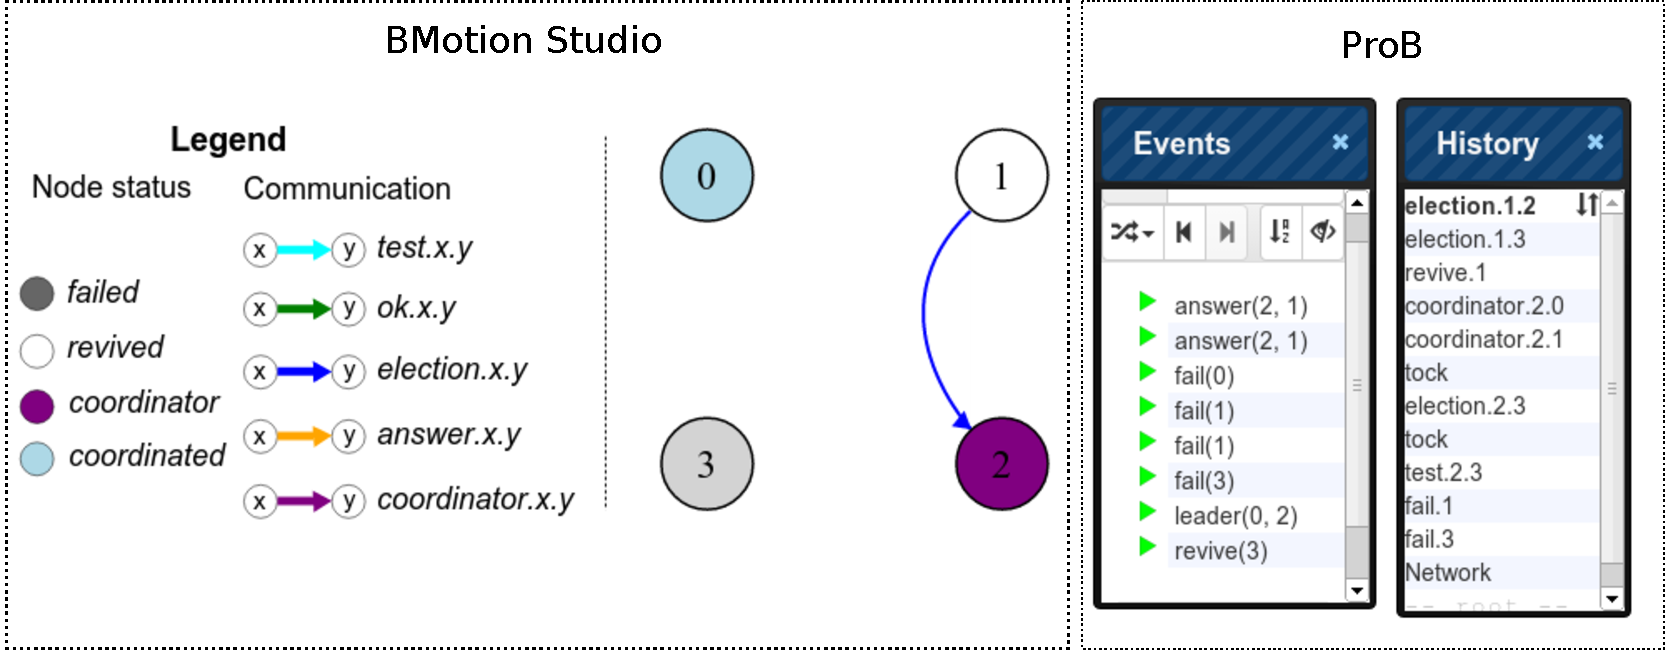
\includegraphics[width=16cm]{img/tutorial/runningvis}
	\caption{The final Bully Algorithm Visualisation}
	\label{fig:BullyVisState}
\end{figure}

In general, we want to visualise the process of electing a leader in the network.
More precisely, we aim to visualise the $Network$ process of the CSP specification.
As the bully algorithm specification is presented for a network with four nodes, we also intend to create a visualization for four nodes (the nodes are enumerated from 0 to 3). 
Fig.~\ref{fig:BullyVisState} demonstrates the visualization of a particular trace.

There are two major aspects of the specification that we want to visualise: the nodes and the communication between the nodes.
Each node is visualised by means of a circle in which the respective ID is positioned, whereas the communication between the nodes is illustrated by directed arrows.
Each directed arrow is made up of a line and a corresponding arrowhead.

To each visual element in the visualization we assign a unique ID referring to the elements in the CSP specification.
Thus, the node with ID $x$ in the CSP specification is presented by the circle with ID "n-x" in the visualization.
Additionally, a message transfer from the node with ID $x$ to the node with ID $y$ is represented by the line with ID "l-x-y" and the arrowhead with ID "p-y" (i.e. the arrow connecting "n-x" and "n-y").
In this section, both symbols $x$ and $y$ stand for an integer ranging from 0 to 3.

We can classify all types of events in the specification into the following groups:
\begin{itemize}
\item \textbf{status:} Events that can change the status of a particular node $x$: $fail.x$, $revive.x$, $coordinator.x.y$, and $leader.x.y$.
\item \textbf{message:} Events illustrating a message transfer from node $x$ to node $y$: $test.x.y$, $ok.x.y$, $election.x.y$, $answer.x.y$, and $coordinator.x.y$.
\item \textbf{hidden:} Events that are not considered in the visualization: $tock$.
\end{itemize}
Thus, we can infer that there are two general types of observers to define: the \textit{status} and the \textit{message} observers.
Note that each \textit{coordinator} event (\textit{coordinator.x.y}) has been included in the first two groups above. 
This is because in the specification each of the \textit{coordinator} events intends to identify the coordinator ($x$) and at the same time represents a message transfer (to node $y$).

The status of a node usually changes when one of the \textit{status} events has been executed.
Each node, except for the node with the lowest ID\footnote{The node with ID 0 can never be a coordinator as there is no node with a lower ID.}, can have the following status: \texttt{failed}, \texttt{revived}, \texttt{coordinator}, or \texttt{coordinated}.
A unique colour has been selected for distinguishing each possible status of a node (see legend in Fig.~\ref{fig:BullyVisState}).
For instance, the node with ID ``n-3'' will be coloured in grey when the event $fail.3$ has been processed.

\subsection{Creating Observers}

Start by adding a new CSP event observer to the visual element that matches the selector ``\#bully''.
Add the following JavaScript code to your \texttt{template.js} file:

\begin{lstlisting}[language=JavaScript]
$("#bully").observe("csp-event", {
  observers: []
});
\end{lstlisting}

The visual element that matches the selector ``\#bully'' defines the parent for the CSP event observer.
In particular, the selector matches the SVG element (the actual visualization) that we added in the previous Section~\ref{tutorial_csp_create_vis}.

In order to associate a \textit{status} event from the CSP specification with a node in the visualization, we use the selector ``\#n-\{\{a1\}\}'' in the definition of the respective observer. 
The construct ``\{\{a1\}\}'' is used in the selector for obtaining the value of the first argument of the respective \textit{status} event.
For example, the observer for changing a status of a node to \texttt{failed} can be defined as follows:

\begin{lstlisting}[language=JavaScript]
{
  exp: "{fail.x | x <- {0..N-1}}",
  actions: [
    { selector: "#n-{{a1}}",
      attr: "fill",
      value: "lightgray"
    }
  ]
}
\end{lstlisting}

\begin{figure}[h!]\centering
	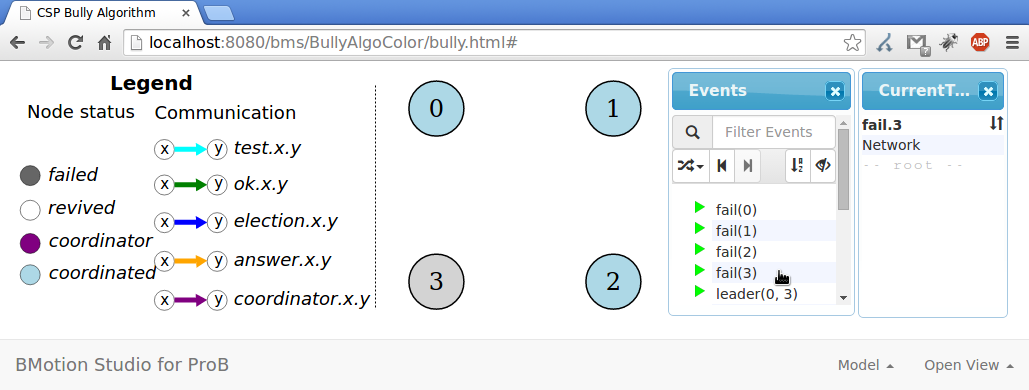
\includegraphics[width=16cm]{img/tutorial/bully1}
	\caption{The Bully Algorithm Visualisation}
	\label{fig:bully1}
\end{figure}

Add this observer to the list of observers.
In line 2 we define the user-defined expression that constitutes the set of observed events.
In this case the expression defines the set of events $\{fail.0, fail.1, fail.2, fail.3\}$ with $N=4$.
Whenever the current processed event is a member of this set, the actions (defined in line 3 to 8) are executed.
In particular, the observer executes only one action that sets the fill attribute of the visual element that matches the selector to lightgray.
Consider line 4: We define the selector based on the value of the first parameter (\{\{a1\}\}) of the current processed event.
For example, if the current processed event is \textit{fail.3}, the selector will be defined as ``\#n-3''.
Refresh your browser and open the ProB Events view (\textsf{Open View $\rangle$ Events}).
Start the \textit{Network} process, execute the \textit{fail.3} event and see that happens with your visualization.
The corresponding node should be coloured in lightgray as demonstrated in Figure~\ref{fig:bully1}.
In a similar fashion we can define the observers for the other node status changes. 

For creating the \textit{message} observers we need to consider both arguments of the \textit{message} events.
The types of the messages are distinguished by different colours (see Figure \ref{fig:BullyVisState}).
Thus, each \textit{message} observer, except for the \textit{coordinator} observer (this observer has three actions), has two actions: one action for appearing the arrow (the line and arrowhead constituting the respective arrow in the visualization) and one action for changing the color of the arrow.
For instance, the observer for visualising the test message can be defined as follows:

\begin{lstlisting}[language=JavaScript]
{
  exp: "{test.x.y | x <- {0..N-1}, y <- {0..N-1}}",
  actions: [
    { selector: "#l-{{a1}}-{{a2}}, #p-{{a2}}",
      attr: "class",
      value: "visible"
    },
    { selector: "#l-{{a1}}-{{a2}}",
      attr: "stroke",
      value: "cyan"
    }
  ]
}
\end{lstlisting}

\begin{figure}[h!]\centering
	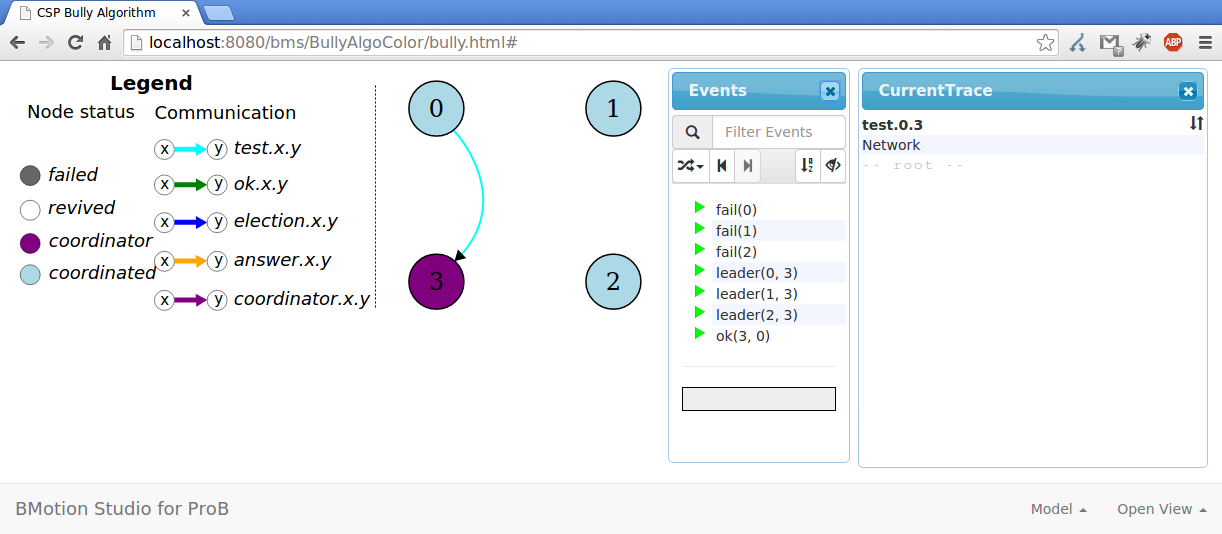
\includegraphics[width=16cm]{img/tutorial/bully2}
	\caption{The Bully Algorithm Visualisation}
	\label{fig:bully2}
\end{figure}

Add the observer to the set of observers.
The first action (line 4 to 7) sets the attribute class to the value ``visible''.
In the next step we need to define the visible and hidden classes respectively.
Add the following code within your head tag in your \texttt{index.html} file:

\begin{lstlisting}[language=html]
<style type="text/css">
  .hidden {
    visible:hidden;
  }
  .visible {
    visible:visible;
  }
</style>
\end{lstlisting}

Refresh your browser and see what happens with your visualization.
For instance, execute the event \textit{test.0.3}.
A directed cyan coloured arrow from node 0 to 3 should be displayed as demonstrated in Figure~\ref{fig:bully2}.
In a similar fashion we can define the observers for the other message types. 

To provide a clear visualization an additional observer has been added to hide all arrows after performing an arbitrary event.
This observer is applied on the currently processed event before all other defined observers:

\begin{lstlisting}[language=JavaScript]
{
  exp: "Events",
  actions: [
    { selector: "path[id^=l-], path[id^=p-]", 
      attr: "class", 
      value: "hidden"
    }
  ]
}
\end{lstlisting}
 
The initial state of the specification and the visualization is the state in the network where all nodes are alive and the coordinator is the node with the ID 3 (the node with the greatest ID). 
Additionally, no message exchanges are performed.

\subsection{Final Visualisation}

You can download the final visualization \file{CSPBullyAlgo.zip}{here}.
\section{Reference}
\label{reference_csp}

\subsection{Observers}
\label{observers_csp}

\subsubsection{Formula Observer}

The formula observer observes a list of formulas (i.e. expressions) and triggers a function whenever a state change occurred.
The result of the formulas are passed to the trigger function.
The following options can be passed:

\begin{tabular}{ l l l p{7cm} }
  \textbf{Name} & \textbf{Type} & \textbf{Default} & \textbf{Description} \\
  \hline\noalign{\medskip}
  formulas & list / function* & empty list & Define a list of expressions that should be evaluated and passed to the trigger function.\\
  \hline\noalign{\medskip}
  cause & string / function* & '\textit{AnimationChanged}' & The trigger cause. Possible values: '\textit{AnimationChanged}', '\textit{ModelChanged}' and '\textit{ModelInitialised}'. \\
  \hline\noalign{\medskip}
  trigger & function &  & The trigger function will be called after every state change with its \textit{origin} reference set to the element that the observer is attached to and the requested \textit{data} (the result of the expressions). \\
\end{tabular}

*This attribute also accepts a function that should return its value.

\begin{lstlisting}[language=JavaScript]
$("#vis").observe("formula", {
  formulas: ["N"],
  trigger: function (origin, data) {
    origin.text(data.values[0].value);
  }
})
\end{lstlisting}

\subsubsection{CSP Event Observer}

The mathematical semantics of CSP are mainly based on \textit{traces}.
A trace is a sequence of events performed by a process that can communicate and interact with other processes within the CSP model.
The basic idea of the CSP visualisation approach is to visualise the information encoded in the given sequence of events (\textit{trace}).
However, a process may perform many different traces and thus creating a visualisation manually for each possible trace is an almost impossible task.

The presented approach requires the user to set up only one visualisation that may be capable of representing any possible trace of a CSP process of a particular model. 
This is achieved by means of \textit{observers}) that are used to link the visualisation with the model.

We extended BMotionWeb with a new observer type called \textit{CSP event observer} in order to support creating visualisations of CSP models.
The observer has the following structure:

\begin{lstlisting}[language=JavaScript]
{ "exp": "<user-defined CSP expression>", 
  "actions": [ 
    { "selector":"<selector>", "attr":"<attribute>", "value":"<value>" },
    { ... }
  ] }
\end{lstlisting}

Each observer has a \textit{user-defined CSP expression} and a list of \textit{actions}.
The user-defined expression constitutes a set of observed events, whereas the actions determine the changes made on visual elements.

An action defines a \textit{selector} that matches a set of visual elements in the visualisation (SVG graphic). 
A selector follows the syntax provided by jQuery\footnote{For more information about jQuery and selectors we refer the reader to the jQuery API documentation \url{http://api.jquery.com/category/selectors/}.}. 
For instance, to match the visual element with the ID ``elem1'' (each element should have a unique ID in the visualisation) the user can define the selector ``\#elem1''. 
The prefix ``\#'' is used for matching a visual element by its ID in jQuery. 
An action also defines an \textit{attribute} (e.g. ``fill'' for colouring the interior of a visual element like a circle shape) and a corresponding \textit{value} that will be set as the new value of the attribute when the action is triggered.
The actions of an observer $o$ are triggered when the currently processed event is in the set of observed events of $o$.

The user can refer to the information given by the arguments of the currently processed event within the action fields (selector, attribute and value).
This is achieved by means of the construct ``\{\{aN\}\}'' where aN refers to the N-th argument of the event.
For instance, if the event has two arguments, then the first and the second one can be obtained with ``\{\{a1\}\}'' and ``\{\{a2\}\}'', respectively. 
To illustrate this, consider an event $evt.x$ with $x \leftarrow 0..4$.
One may want to use the information given by the first argument $x$ of $evt$ within a selector in order to match visual elements that have an ID of the form ``elem$x$''.
This can be done by defining the selector ``\#elem\{\{a1\}\}''.
The construct ``\{\{a1\}\}'' will be replaced by the value of the first argument of the currently processed event in the observer.
For instance, if the currently processed event is $evt.2$, the selector ``\#elem\{\{a1\}\}'' will become ``\#elem2''.

\begin{figure}[h!]\centering
	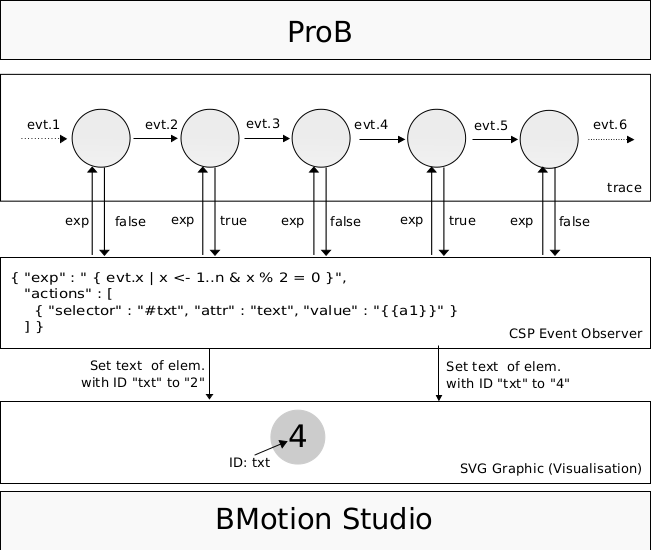
\includegraphics[width=14cm]{img/reference/detailprocess}
	\caption{The function of the CSP event observer}
	\label{fig:detailprocess}
\end{figure}

Fig.~\ref{fig:detailprocess} illustrates the function of the CSP event observer on a simple example.
The visualisation consists of an SVG graphic with a text field element with the ID ``txt'' and one CSP event observer.
The CSP event observer defines an expression that constitutes the set of observed events $evt = \{evt.2, evt.4, evt.6, ..\}$ and one action $act1$ that changes the value of the attribute "text" to ``\{\{a1\}\}'' of the visual element with the ID ``txt'' (the text field).
The observer is executed for each event of a given trace.
This means that, whenever the currently processed event is in the set of observed events $evt$, the observer will trigger the defined action $act1$.
For instance, the execution of the event $evt.4$ causes the observer to set the value of the text field element to ``4'' as demonstrated in Fig.~\ref{fig:detailprocess}.

In general the observer is attached to a parent visual element.
The actions of the observer are applied on the children.
The following options can be passed:

\vspace{0.5cm}
\begin{tabular}{ l l l p{7cm} }
  \textbf{Name} & \textbf{Type} & \textbf{Default} & \textbf{Description} \\
  \hline\noalign{\medskip}
  selector & string / function* & & The selector that matches the parent visual element. \\
  \hline\noalign{\medskip}
  cause & string / function* & '\textit{AnimationChanged}' & The trigger cause. Possible values: '\textit{AnimationChanged}', '\textit{ModelChanged}' and '\textit{ModelInitialised}'. \\  
  \hline\noalign{\medskip}
  observers & list & empty list & Define a list of CSP event observers. \\
  \hline\noalign{\medskip}
  : exp & string / function* & & The user-defined expression that constitutes a set of observed events.\\
  \hline\noalign{\medskip}
  : actions & list & & A list of actions that should be applied on the visual elements. \\
  \hline\noalign{\medskip}
  :: selector & string / function* & & The \textit{selector} matches a set of visual elements. \\
  \hline\noalign{\medskip}
  :: attr & string / function* & & The attribute that should be modified. \\
  \hline\noalign{\medskip}
  :: value & string / function* & & The value that should be set on the attribute. \\
\end{tabular}

*This attribute also accepts a function that should return its value.

\begin{lstlisting}[language=JavaScript]
$("#crossing").observe("csp-event", {
  observers: [
    { exp: "{gate.down,gate.up}",
      actions: [
        {selector: "g[id^=gate]", 
        attr: "opacity", 
        value: "0"}
      ]
    },
    { exp: "{gate.down}",
      actions: [
        {selector: "#gate-go_down-2, #gate-go_down-1", 
         attr: "opacity", 
         value: "100"}
      ]
    },
    { exp: "{gate.up}",
      actions: [
        {selector: "#gate-go_up-2, #gate-go_up-1", 
        attr: "opacity", 
        value: "100"}
      ]
    },
    { exp: "{enter.x.y | x <- {0..4}, y <- {Train1,Train2}}",
      actions: [
        {selector: "#train_{{a2}}", 
        attr: "x", 
        value: "{{a1}}00"},        
        {selector: "#train_{{a2}}", 
        attr: "transform", 
        value: ""}
      ]
    },
    { exp: "{leave.x.y | x <- {0..3}, y <- {Train1,Train2}}",
      actions: [
        {selector: "#train_{{a2}}", 
        attr: "transform",
        value: "translate(50,0)"}
      ]
    }
  ]
});
\end{lstlisting}

\chapter{Frequently Asked Questions}
\label{faq}

\section{General Questions}

\subsection{What is BMotion Studio?}

Text ...


\clearpage
\phantomsection
\addcontentsline{toc}{chapter}{Index} 
\printindex

\end{document}

